\documentclass{article}
% Load Package
\usepackage{blindtext}
\usepackage{graphicx}
\usepackage{multicol}
\usepackage{tabularx}
\usepackage{booktabs}
\usepackage{pgffor}
\usepackage{color}
\usepackage[hyperfootnotes=true,colorlinks=true,allcolors={blue}]{hyperref}
\usepackage{indentfirst}
\usepackage{dcolumn}
\usepackage{nameref}
\usepackage{placeins} % put this in your pre-amble
\usepackage{flafter}  % put this in your pre-amble
\usepackage{float} % to manage figure float
\usepackage{authblk} % for co-author
\usepackage{dirtytalk} % for inserting quotation
\usepackage{siunitx} % for the \nombre command
%\usepackage{cite}
\usepackage{bookmark}
%\usepackage{lmodern}
%\usepackage{mathptmx} % for nice font
%\fontfamily{cmss}
\usepackage{mathtools}
% \hypersetup{
%   colorlinks=true,
%   allcolors=blue
% }

\usepackage{threeparttable}
\usepackage{booktabs, longtable}
\usepackage{tabularx}
\usepackage[singlelinecheck=false]{caption}
% for source under image
\usepackage{caption}
%\newcommand{\source}[1]{\fontsize{7}{8}\selectfont Source: {#1}}
\newcommand{\source}[1]{\caption*{\fontsize{7}{8}\selectfont Source: {#1}} }

% for accessibility 
\newcommand{\alt}[1]{\caption*{\fontsize{9}{11}\selectfont Alt text: {#1}} }


%\input{../shared/statex}


%\usepackage{amssymb} %maths
%\usepackage{amsmath} %maths
%\usepackage{siunitx} % using plus-minus instead of std
\DeclareUnicodeCharacter{2212}{-} % Unicode U+2212 is MINUS SIGN, which is not set up by default with inputenc
\DeclareUnicodeCharacter{2009}{~} % Unicode U+2212 is MINUS SIGN, which is not set up by default with inputenc{00A0}{~}

\DeclareUnicodeCharacter{0080}{+} % Unicode U+2212 is MINUS SIGN, which is not set up by default with inputenc{00A0}{~}

\DeclareUnicodeCharacter{0301}{-} % Unicode U+2212 is MINUS SIGN, which is not set up by default with inputenc{00A0}{~}

\DeclareUnicodeCharacter{0301}{+} % Unicode U+2212 is MINUS SIGN, which is not set up by default with inputenc{00A0}{~}

\DeclareUnicodeCharacter{0300}{-} % Unicode U+2212 is MINUS SIGN, which is not set up by default with inputenc{00A0}{~}

\DeclareUnicodeCharacter{0300}{+} % Unicode U+2212 is MINUS SIGN, which is not set up by default with inputenc{00A0}{~}

\DeclareUnicodeCharacter{001B}{-} % Unicode U+2212 is MINUS SIGN, which is not set up by default with inputenc{00A0}{~}

% Count of words
\usepackage{moreverb} % for verbatim ouput
\immediate\write18{texcount  -inc -merge -nobib -sum -sub=section \jobname.tex > ./texcount.tex}
\newcommand\wordcount{\verbatiminput{./texcount.tex}}

% font family and size
\usepackage{CormorantGaramond}
%\usepackage[default]{gillius}

%\usepackage{anyfontsize}
%\fontsize{15}{18}\selectfont
\usepackage[fontsize=13]{scrextend}
%\usepackage[14pt]{extsizes}


% page setup
\usepackage{geometry} % for margin
\geometry{
  left=25mm,
  right=25mm,
  top=25mm,
  bottom=25mm,
  heightrounded,% better use it
}


\usepackage{url}
\usepackage[style=apa,backend=biber,url=false,doi=false,natbib]{biblatex}
\addbibresource{src/ref.bib}


\makeatletter
\newcommand{\myfnsymbol}[1]{%
  \expandafter\@myfnsymbol\csname c@#1\endcsname
}
% Mapping of how the symbols will be interpreted sequentially
\newcommand{\@myfnsymbol}[1]{%
  \ifcase #1
    % 0
  \or 1% 1
  \or 2% 2
  \or 3% 3
  \or \TextOrMath{\textasteriskcentered}{*}% 4
  \or \TextOrMath{\textdagger}{\dagger}% 5
  \fi
}

\newcommand{\affiliationA}{\@myfnsymbol{1}}
\newcommand{\affiliationB}{\@myfnsymbol{2}}
\newcommand{\affiliationC}{\@myfnsymbol{3}}
\newcommand{\equalcontributor}{\@myfnsymbol{4}}
\newcommand{\correspondingA}{\@myfnsymbol{5}}
\makeatother

\title{\textbf{Estimating the Influence of Demographic Ageing and Migration to the Spanish Aggregate Labour Supply}}

\author{
  Gilbert Montcho\textsuperscript{\affiliationA,\equalcontributor},
  Alejandro Steven Fonseca-Zendejas\textsuperscript{\affiliationB,\equalcontributor,\correspondingA},
  Marcel Mérrete\textsuperscript{\affiliationC,\equalcontributor}
}

\begin{document}


\renewcommand{\thefootnote}{\myfnsymbol{footnote}}
\maketitle

% Layout the notes in order
\footnotetext[1]{Department of Demography, University of Montreal, Montreal, Quebec, Canada}%
\footnotetext[2]{Department of Economics, Universidad Loyola Andalucía, Seville, Spain}%
\footnotetext[3]{Department of Economics, University of Ottawa, Ontario, Canada}%
\footnotetext[4]{All authors contributed equally}%
\footnotetext[5]{Corresponding author: asfonseca@uloyola.es}%

\setcounter{footnote}{0}% Restart footnote counter
% Footnotes for rest of document uses \fnsymbol 
\renewcommand{\thefootnote}{\fnsymbol{footnote}}

% show abstract on the title page
\begin{abstract}

Population aging has raised concerns about its impact on the labor supply. However, quantifying these effects often focuses only on the increase in the elderly population, at the expense of the working age groups. This article estimates the aggregate labor supply in Spain and examines the extent to which population aging, immigration, and individual behaviors have contributed to its growth between 2006 and 2023.

\vspace{0.7em}\par
\textbf{Keywords}: Labour Supply, Immigration, Populating Ageing, Decomposition Models.
\end{abstract}
\newpage
  % show table of content on esparate page
  {\fontsize{13pt}{13}
    \selectfont
      \tableofcontents
  }
  
  % load content
  \newpage

%%%%%%%%%%%%%%%%%%%%
\section{Introduction and Litterature}

Across the countries of Western Europe, Spain is a representative case that exhibits two major phenomena that currently concern policymakers: population ageing and immigrant inflows. These conditions result in several economic and social outcomes. From an initial standpoint, it is widely recognized that there are side-effects to an ageing society, which are evident in social security finances under substantial stress affecting PAYG systems \citep{ diaz2009delaying,boeri2024pay}, increments in public expenditure on health services \citep{cristea2020impact, aiyar2016impact, bijak2007population}, and social security \citep{failde2021perspective}. Furthermore, the ageing population impacts the labour market as there exist a decline in labour force \citep{maestas2023effect}. Concerning the labour market in Spain, \citep{casares2018labor}, demonstrated that labour force shocks are more persistent, and this labour force growth can be explained by separate factors and one such factor is the influx of a substantial number of non-EU immigrants. This suggest that immigration influences the Spanish aggregate labour supply besides the age structure of the population. \\

As a result, several investigations have suggested that replacement migration is proposed as a strategy to alleviate the effects of ageing because it assists in easing downturns in labour supply, boost competitiveness and fosters economic growth \citep{stepanek2022sectoral, okamoto2021immigration, UNATIONS}. However, the expansion of working population and, therefore, the increase in public revenues, migration also creates additional needs for public services. Consequently, migration affects both the tax and the welfare system \citep{fiorio2023migration, naumann2021population}. For example, as stated in \citep{ preston2014effect},immigration can result in costs by the utilization of public services but can also influence the expense of offering services to natives. Having said that, in developing countries, extended individual longevity or population ageing and migration are among the most significant challenges \citep{ciobanu2020intersections}. \\

As summarized previously, the impacts of population ageing, and migration are multifaceted, and an all-encompassing solution does not address every situation. Therefore, handling these matters requires a targeted approach. As a result of this, an examination of the combined effects and potential benefits on the aggregate labour supply by demographic ageing is carried out in this paper. This analysis is conducted understanding that demographic ageing is driven by joint effects of fertility rates, mortality rates, and, certainly, immigration patterns. Thus, it becomes feasible to estimate the aggregate labour supply and analyse the impact of immigration in Spain over time. 


\subsection*{Origins and Status of Immigration and Ageing in Spain}


\section{Data Source and Methodology}\label{sec:lab_method}

  \subsection{Measuring the Aggregate Labor Supply}
  Aggregate labor supply \(L\) is estimated by the weighted sum of hours worked during the year by age \(a\) and by residence status \(r\) (\(whx_{ar}\)), with \(r = (\text{immigrant, native})\). 

  The weighting factor is the product of the total population size (\(pop_{r}\)), the population structure (\(str_{ar}\)), and the labor participation rates (\(wpx_{ar}\)) by age and residence status.

  \begin{equation}\label{eq:pclab}
    L = \displaystyle\sum_{r}\displaystyle\sum_{a}(pop_{r} \times str_{ar} \times wpx_{ar} \times whx_{ar}) = f(pop_{r}, str_{ar}, wpx_{ar}, whx_{ar})
  \end{equation}


  \subsection{Data sources and descriptives}


  \subsection{The Model of Continuous Change}
  
  To measure the isolated effect of demographic aging on the aggregate labor supply, the continuous change model \citep{horiuchiDecompositionMethodBased2008} was used. This model allows decomposing the difference between two summary measures resulting from the same process into several components, each representing the contribution of underlying factors to the process. The process is a function \(f\), taking as arguments the values of the factors (covariates or independent variables) and returning a summary measure (the dependent variable or variable of interest).
  
  \vspace{0.7em}\par
  \citet{horiuchiDecompositionMethodBased2008} demonstrates that as the factors transition from values \(x_i(t_1)\) to \(x_i(t_2)\) between two times \(t_1\) and \(t_2\), the summary measure changes from \(f(x_i(t_1))\) to \(f(x_i(t_2))\), and the difference between these two measures can be decomposed into additive components \(c_{i}\) representing the contribution of changes within each factor to this difference. This is expressed by equation \eqref{eq:hofr}.
  
  \begin{equation} \label{eq:hofr}
    f(x_i(t_2)) - f(x_i(t_1)) = \displaystyle\sum_{i}c_{i}
  \end{equation}
  
  \vspace{0.7em}\par
  With \(i = 1, 2, ..., n\) being the factors involved. The decomposition is based on the assumption that the change in the covariate \(x_i\) occurs continuously or gradually over a real or hypothetical time dimension \(t_1 \rightarrow t_2\). This provides a reasonable justification for the additivity of the effects of the factors and the elimination of interaction terms even if the process in question is a non-additive function of the covariates \citep[p.~786]{horiuchiDecompositionMethodBased2008}.
  
  \vspace{0.7em}\par
  In other words, the continuous change model (CCM) introduces a decomposition function \(g\) which, using a process function \(f\), transforms two series of covariates, the vectors \(X(t_1)\) and \(X(t_2)\) representing the values of the covariates \(X = (x_1, ..., x_i, ..., x_n)\) at times \(t_1\) and \(t_2\), into a series of contributions or effects, the vector \(C = (c_1, ..., c_i, ..., c_n)\). Thus, we can write:
  
  \begin{equation}\label{eq:gfr}
    C = g(X, f)
  \end{equation}
  
  The series \(X\) and \(C\) having the same lengths, results in a perfect correspondence between the factors and the effects, which can be grouped for analysis purposes. Furthermore, the idea of continuity implies that each element \(c_i\) of the series \(C\) is obtained by integration according to the equation:
  
  \begin{equation}\label{eq:mxfr}
    c_i = \int_{x_i(t_1)}^{x_i(t_2)} \frac{\partial f(t)}{\partial x_i(t)} dx_i(t)
  \end{equation}
  
  In practice, equation \eqref{eq:mxfr} is estimated by numerical integration where \(\int_{x_i(t_1)}^{x_i(t_2)} d(t)\) is approximated by \(\sum_{x_i(t_1)}^{x_i(t_2)} \delta(t)\), with \(x_{it} = x_i(t)\) being the value of a factor \(i\) at a moment \(t\). Adapting the continuous change model to measure equation \eqref{eq:pclab} allowed the total variation in the aggregate labor supply between 1981 and 2016 to be distributed not only among these three components but also by age group and residence status (immigrants and natives). For this article, the decomposition was performed by creating an auxiliary function \(g\) around the R package \citep{Rstat:2018} DemoDecomp \citep{DemoDecomp:2018}. The code and data used are available upon request.
  
  \vspace{0.7em}\par
  The CCM model is a better alternative to the standardization method often used in demography to account for differences in population structure when comparing demographic measures. Indeed, standardization requires a third population to serve as a standard, making it somewhat less robust as different standards can lead to different results. The CCM model solves this problem and allows for direct decomposition without interaction terms between the different factors.
  
  Interaction effects in regression analysis refer to situations where the impact of one variable on a dependent variable is not constant or additive but depends on the values of other variables. In traditional decomposition methods, such as standardization, any discrepancy between the overall change and the sum of the individual effects of the variables is also called an interaction effect. In such cases, the interaction represents an incomplete separation of the contributions of individual covariates to the overall change or difference in a dependent variable.

\section{Results and Analysis}

\begin{figure}[H]%
    \caption{Average participation rate by major age groups for immigrants and natives, Spain 2006-2023}
    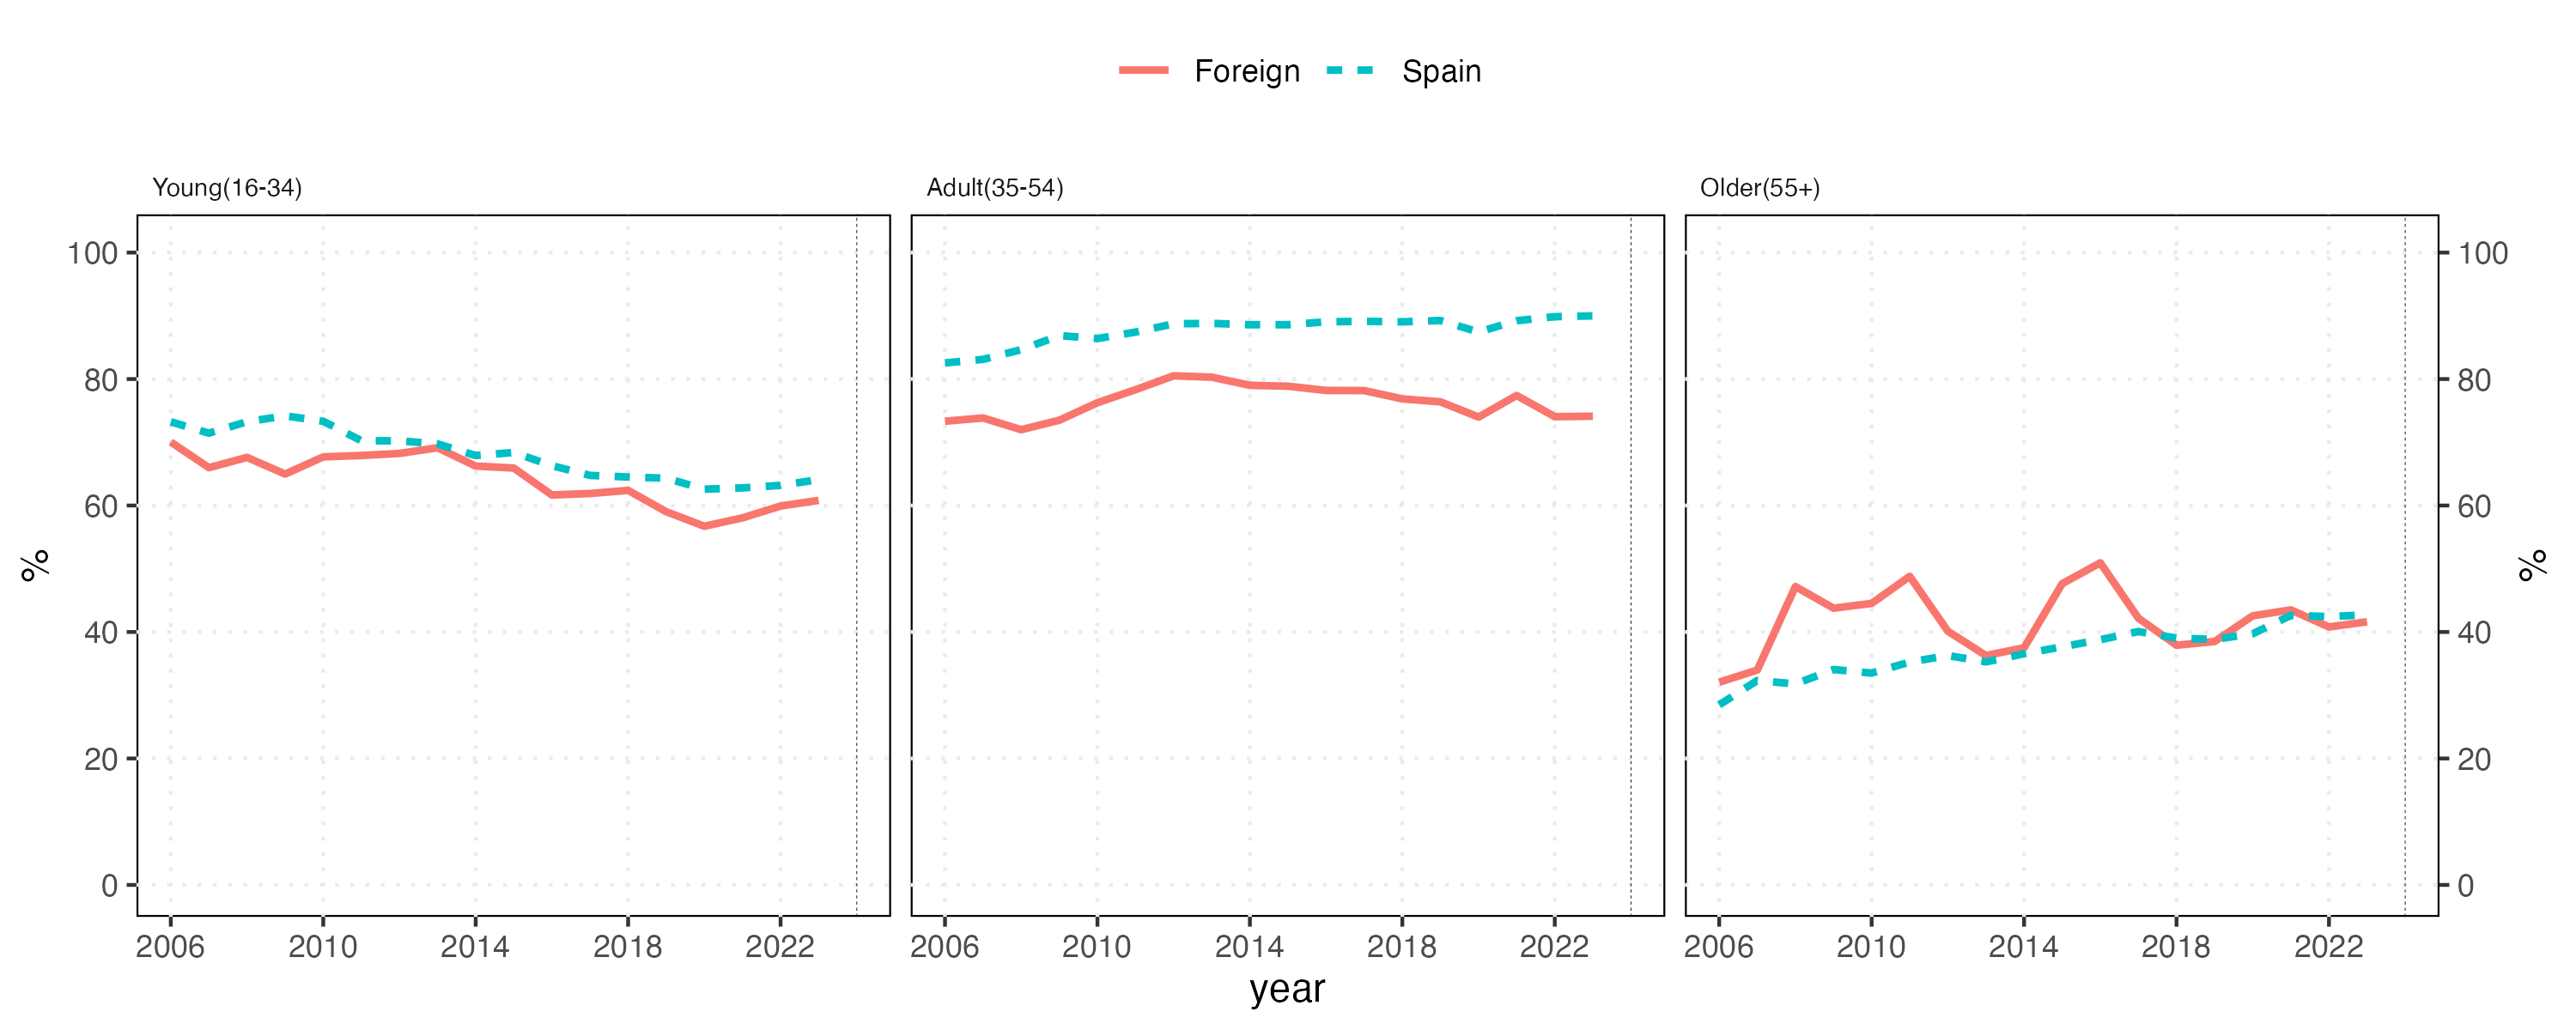
\includegraphics[width=1\textwidth]{../graph/wpx.png}%
    \label{fig:labDecomp}%
\end{figure}%
  


\begin{figure}[H]%
    \caption{Average worked hours by major age groups for immigrants and natives, Spain 2006-2023}
    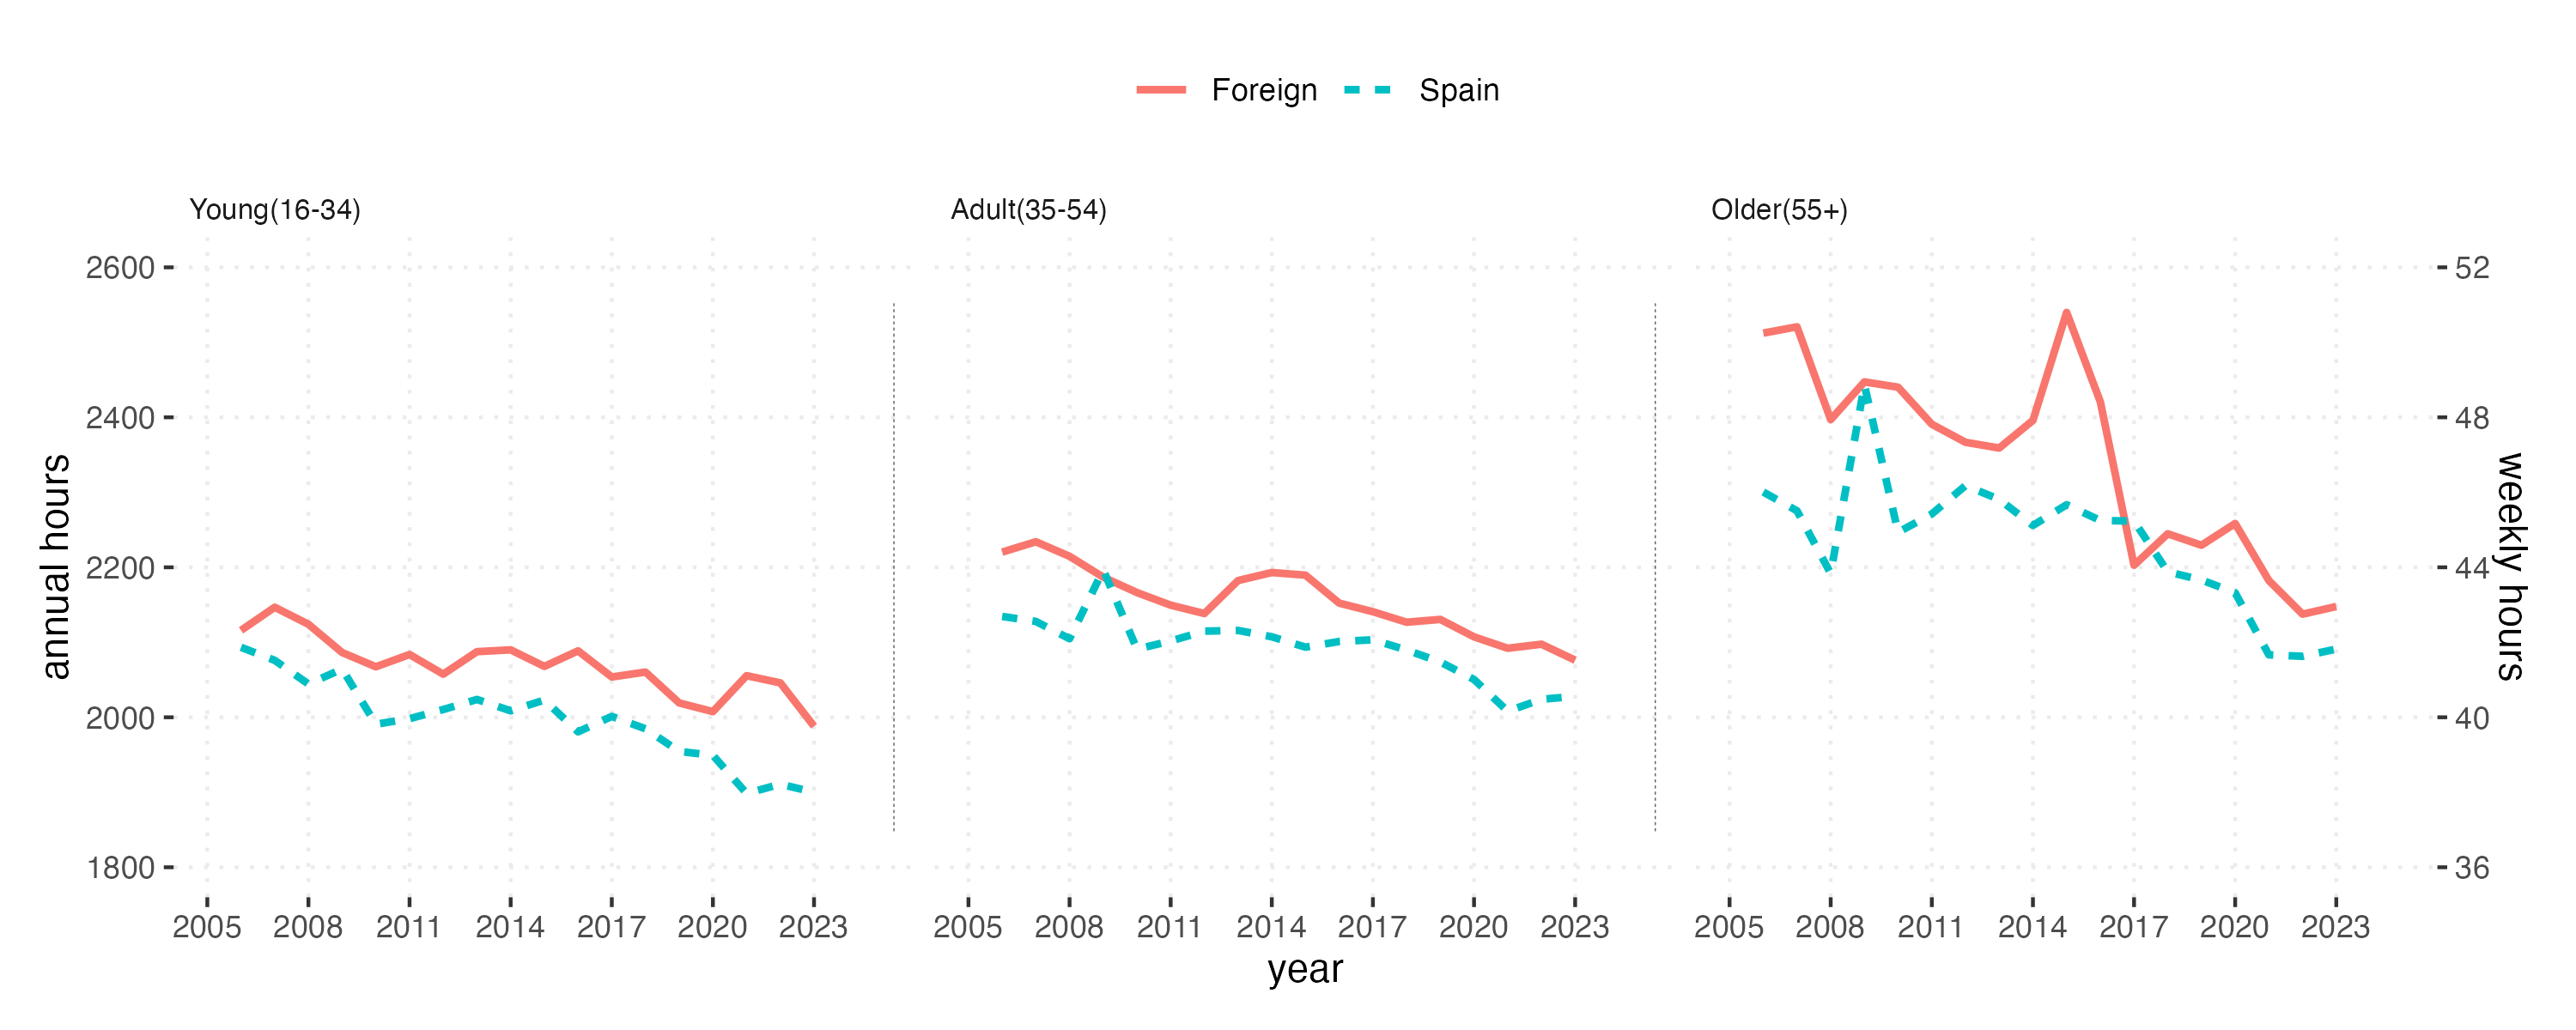
\includegraphics[width=1\textwidth]{../graph/whx.png}%
    \label{fig:labDecomp}%
\end{figure}%

\begin{figure}[H]%
    \caption{Percentage of total population by major age groups for immigrants and natives, Spain 2006-2023}
    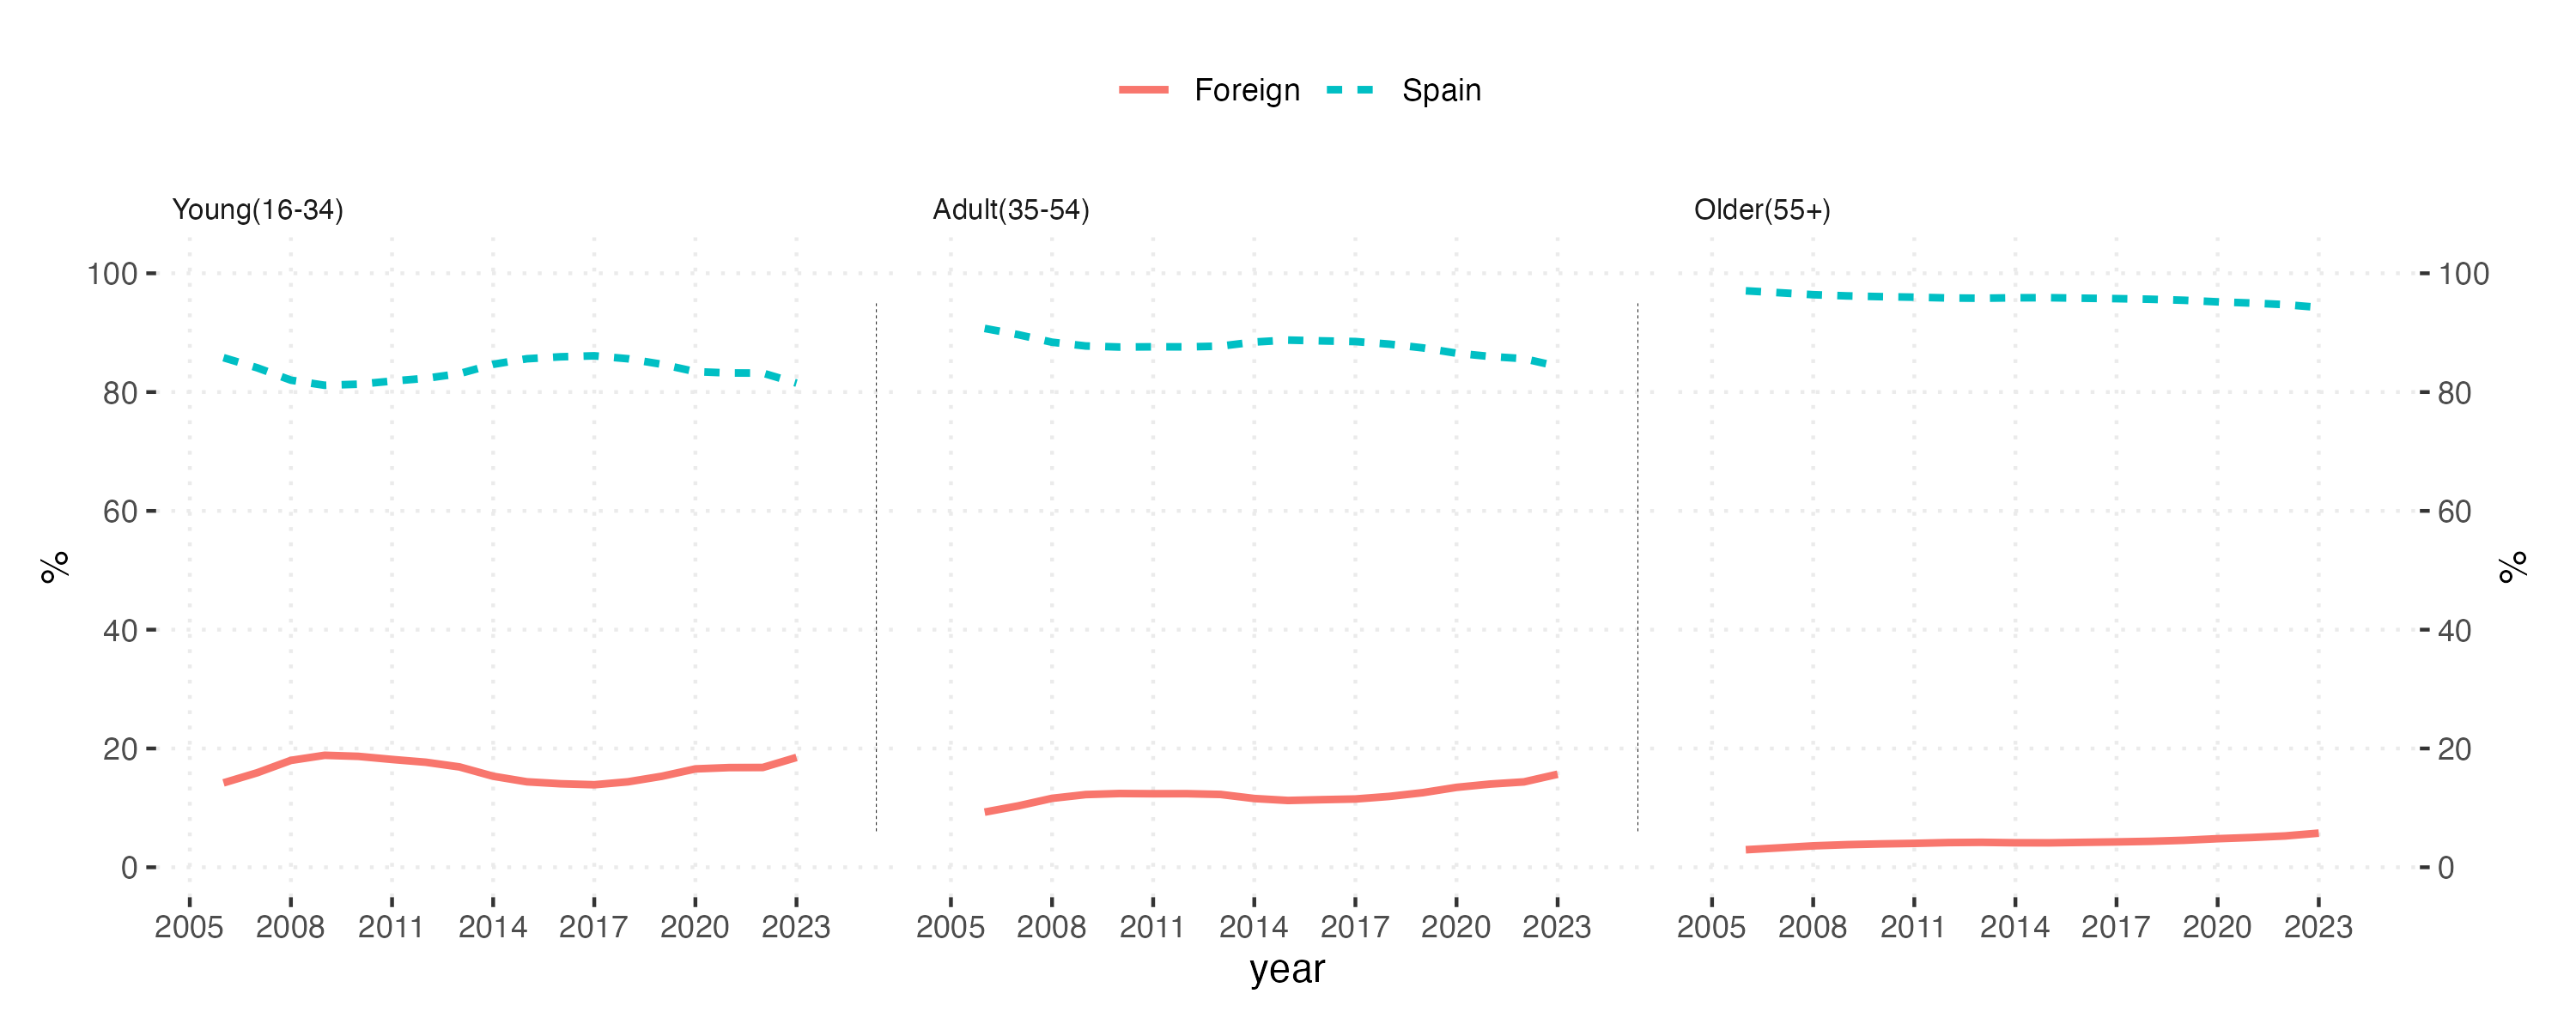
\includegraphics[width=1\textwidth]{../graph/stx.png}%
    \label{fig:labDecomp}%
\end{figure}%
\section{Discussion and Conclusion}







% reference
\section*{Réferences}
%\addcontentsline{toc}{section}{References}
\printbibliography[heading=none]

\end{document}
